\documentclass{article}
\usepackage[utf8]{inputenc}
\usepackage[pdftex]{graphicx}
\usepackage{gensymb}
\usepackage[letterpaper, margin=1in]{geometry}
\usepackage{setspace}
\onehalfspacing


\begin{document}

\begin{titlepage}
    \begin{center}
        \vspace*{1cm}
 
        \Huge
        \textbf{Real Estate Investment Opportunities in the GTA}
 
        \vspace{0.5cm}
        \LARGE
        Capstone Report
 
        \vspace{1.5cm}
 
        \textbf{Jonathan Densil}
 
        \vfill
 
 
        \vspace{0.8cm}
 
        
\includegraphics[width=0.4\textwidth]{ibm.png}
        
        \Large
        IBM Data Science Professional Certificate\\
        Coursera Inc.\\
        \today
 
    \end{center}
\end{titlepage}


\tableofcontents

\newpage

\section{Introduction}

The Greater Toronto Area (GTA) is the most populous metropolitan area housing around 20\% of the population of Canada. Serving as the anchor of the GTA, the second-largest financial sector in North America. Toronto is the 4\textsuperscript{th} largest city in North America and Canada's business and financial capital. The GTA also has nearly 100,000 new immigrants annually and 130 million people within a 500 mile radius; such a large flux of people would provide ample real estate investment opportunities (https://torontoglobal.ca/Discover-Toronto-region/Toronto-region-quick-facts).   

\begin{figure}[h]
	\centering
	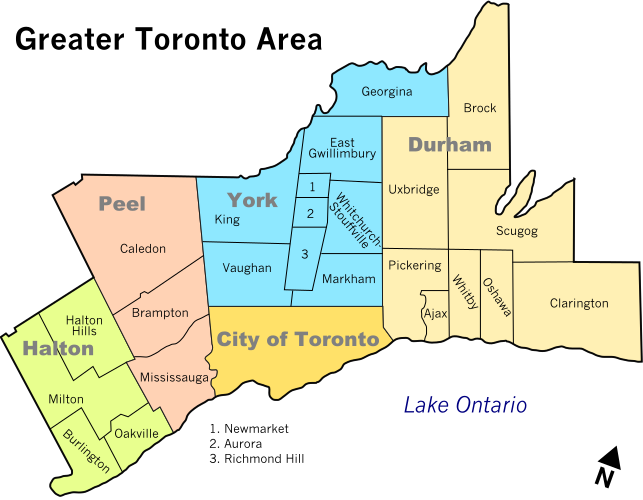
\includegraphics[width=0.8\textwidth]{gta_map.png}
	\caption{Municipalities in the GTA}
	\label{gta}
\end{figure}


\section{Business Problem}

As the old adage goes: location, location, location. Using machine learning and artificial intelligence to determine the best locations to buy a home or commercial real estate will be a key tool for realtors in advising clients of where to invest. Developing this kind of model would also be of great value to immigrants and internal migrants seeking to buy a home in an new and unknown location, giving them a sense for the community before committing to a life-changing decision.

\clearpage
\section{Data}

In order to create the dataset needed to train the machine learning algorithm, we will need the following data:

\begin{itemize}
	\item Real estate sales in Ontario to determine a range of affordability options
	\item Popular venues and attractions that will potentially raise the house prices and attract traffic
	\item Geolocation data to visualise the potential areas of interest  
\end{itemize}

Housing sales data was taken from a kaggle dataset (https://www.kaggle.com/mnabaee/ontarioproperties) since the Canadian Real Estate Association (CREA) prohibits the publication of any analyses, graphs, charts, results, conclusions or forecasts of the MLS\textsuperscript{\textregistered} House Price Index (HPI) data without the prior written consent of CREA (https://www.crea.ca/hpi-tools-terms-of-use/). Geolocation location was taken from the respective municipality open data sources and popular venue data was queried using the Foursquare API. 

\section{Methodology}

Real estate sales data for Ontario was obtained from a Kaggle dataset since the CREA would allow for the publication of any analysis of their data. Once the data had been procured and cleaned, it was plotted to see the distribution. 

\begin{figure}[h]
	\centering
	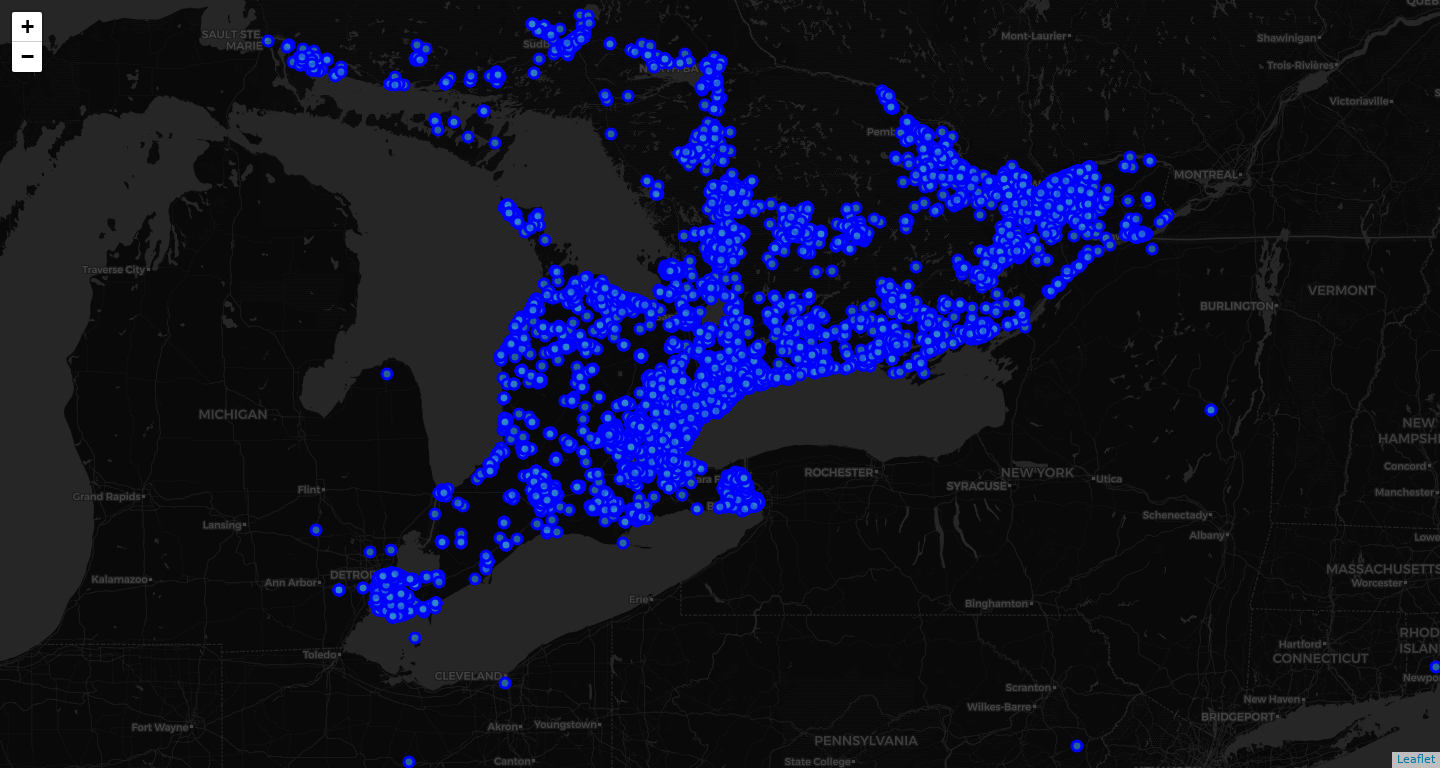
\includegraphics[width=\textwidth]{houses_map.png}
	\caption{Houses in Ontario}
	\label{houses}
\end{figure}

As can be seen in figure \ref{houses}, the majority of the data is not located in the GTA, with some points even in the United States. In order to try and restrict the points to just the GTA, a box with the maximum and minimum values for the latitude and longitude was used to filter the data. 

\begin{figure}[h]
	\centering
	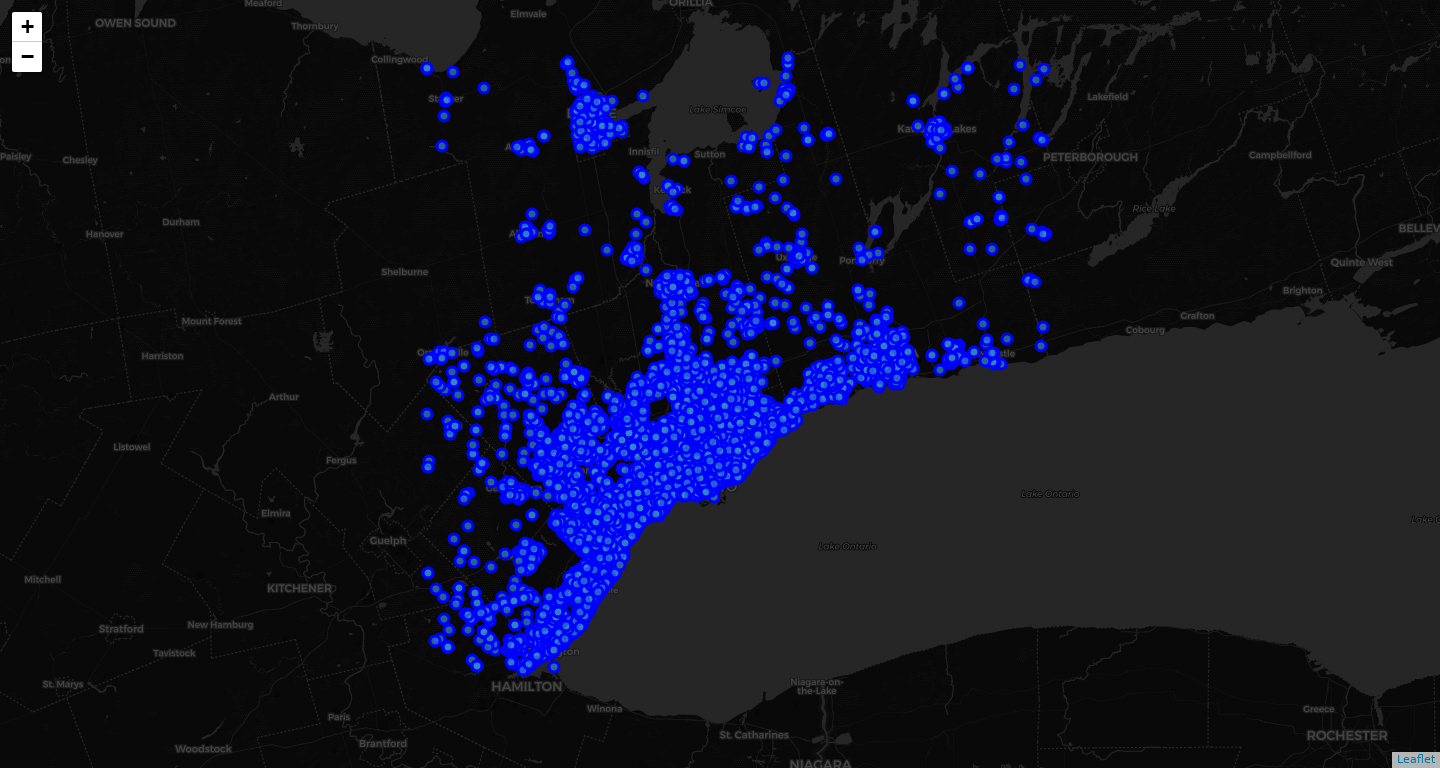
\includegraphics[width=\textwidth]{gta_houses_map.png}
	\caption{Houses in the GTA}
	\label{gta}
\end{figure}

The average housing price data was plotted against each area to see where the pricing distribution falls as seen in figure \ref{price} in the Appendix. An interesting conclusion is that average housing prices for Appleby and especially Bridle Path increase in an exponential fashion. From the Canadian Business, Bridle Path is Canada's richest neighbourhood with an average annual household income of nearly \$1,000,000, and rightly so as the average house price is over \$15,000,000. The rest of the neighbourhood house prices decay in a sort of logarithmic decay. 

The Foursquare API was used to obtain the top 100 most popular venues in a 1.2 km radius. According to the Walk Score corresponds to a 15 minute walk (https://www.walkscore.com/methodology.shtml), which is at a close enough distance to influence the price of housing in the area. For example, if a new mall was built 15 minutes from a condo, its value will increase. 

All the Foursquare venue data was then one-hot encoded into a matrix to be merged with the housing data to be fed into the machine learning algorithm. The k-means algorithm was chosen to carry out the unsupervised clustering algorithm due to its efficiency and easy of computation. The following parameters were fed into the k-means algorithm:

\begin{itemize}
	\item House price
	\item Latitude and longitude
	\item Total venue distance
	\item One-hot encoded venue matrix
\end{itemize}

The location data and total venue distance were also included in order train the model to recognise that the geographic locations also influence the house price. For example, a house in Oakville will cost more than a house in Acton ceteris paribus; this is because it is located in a more upscale neighbourhood. This will also allow the model to distinguish between downtown houses and suburban houses since the total venue distance to the top location will be much less in downtown.  

In order to the find the best k-value to use in the k-means clustering algorithm, three evaluation metrics were used: the Silhouette Coefficient, Calinski-Harabasz Index, and the Davies-Bouldin Index. These three evaluation metrics are useful in determining how well the k-means algorithm clustered if no ground-truth is available. By running these metric for various k values, you can find the optimal k value that would most accurately cluster the data.

The silhouette coefficient is one of the most popular internal evaluation metrics used to evaluate the accuracy of unsupervised learning algorithms, especially density based clustering algorithms. The metric takes into account the mean distance between a sample and all other points in the cluster, and the mean distance between a sample and all other points in the nearest cluster. The higher the score ( max. 1), the higher the density and better the separation between clusters. 

\begin{figure}[h!]
	\centering
	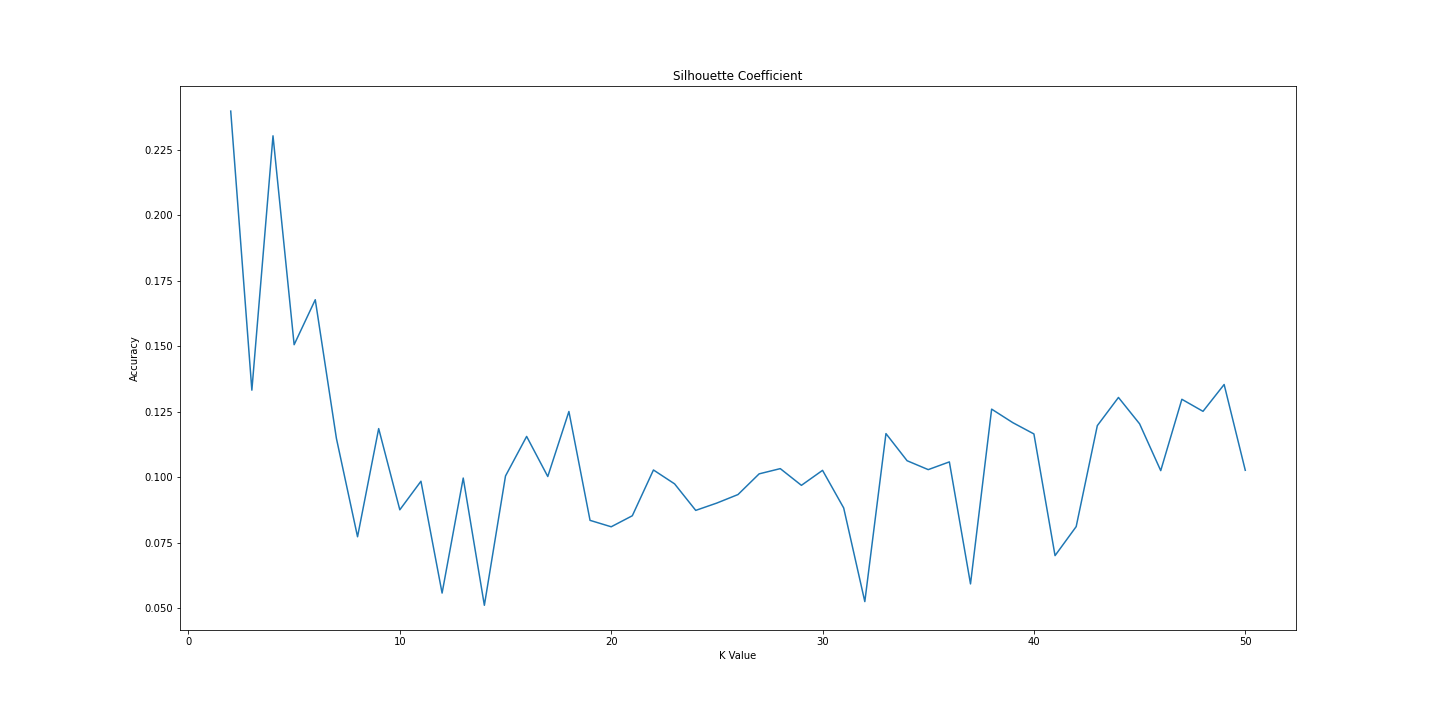
\includegraphics[width=0.9\textwidth]{sil.png}
	\caption{Silhouette Coefficient}
	\label{sil}
\end{figure}

Although the highest accuracy is given by k = 2 as seen in figure \ref{sil}, this would too simply describe the data as it would only point to downtown housing and suburban housing. Therefore, the k value with the second most accurate number of clusters is k = 4. This will provide more insight into the data.

The Calinski-Harabasz Index, also known as the Variance Ration Criterion, is also an internal evaluation metric used to evaluate clusters where no ground-truth labels are available. A higher index relates to a more densely packed cluster with good separation between clusters. 

\begin{figure}[h!]
	\centering
	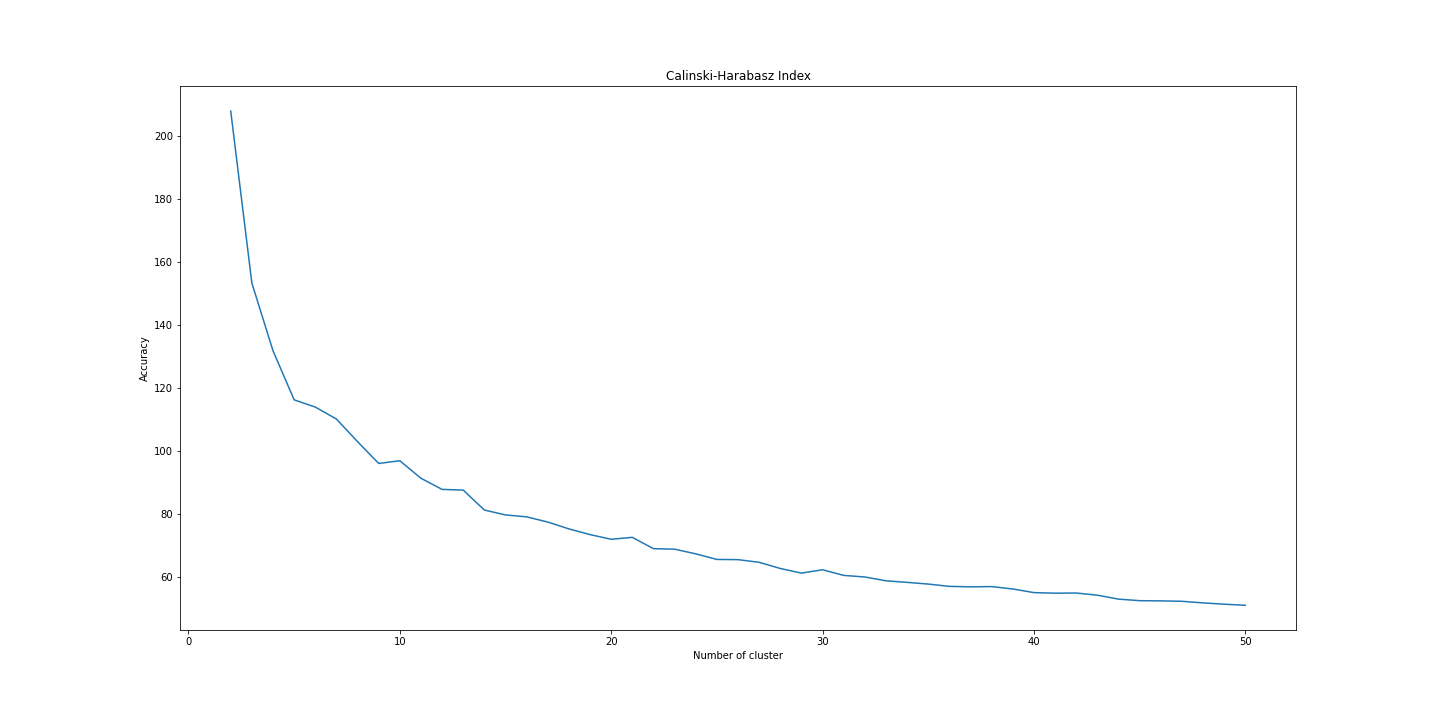
\includegraphics[width=0.9\textwidth]{ch.png}
	\caption{Calinski-Harabasz Index}
	\label{ch}
\end{figure}

The Davies-Bouldin Index, sometimes referred to as the Dunn Index, is an internal evaluation metric for unsupervised clustering algorithms. The index quantifies the average similarity between clusters. Naturally, you would want the similarity to be near zero to have the most distinct and well separated clusters.


\begin{figure}[h!]
	\centering
	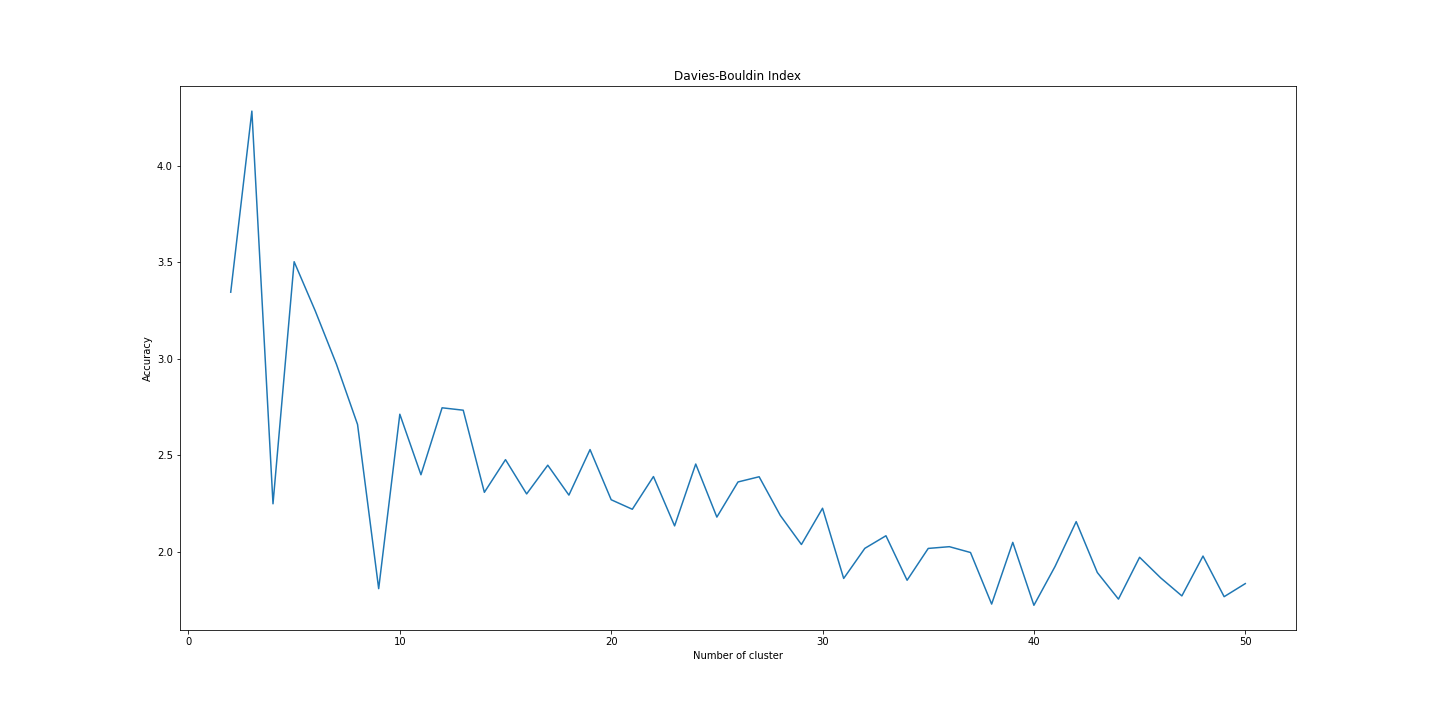
\includegraphics[width=0.9\textwidth]{dunn.png}
	\caption{Davies-Bouldin Index}
	\label{dunn}
\end{figure}

 Contrary to the previous metrics mentioned above, Davies-Bouldin Index is the only one in which the accuracy tends to increase with increasing clusters. This is conceivable because the more discretised the clusters become, the more different they become with one another. By only following the Davies-Bouldin Index, you may risk over-fitting the data by using too many clusters. But, in this case, there is a sharp dip at k = 4, indicating a more accurate representation of the data as compared with k = 2, 3, or even 5.
 

\clearpage
\section{Results}

The k-means algorithm was rerun with k = 4. The following two maps show the distribution of the cluster labels.

\begin{figure}[h]
	\centering
	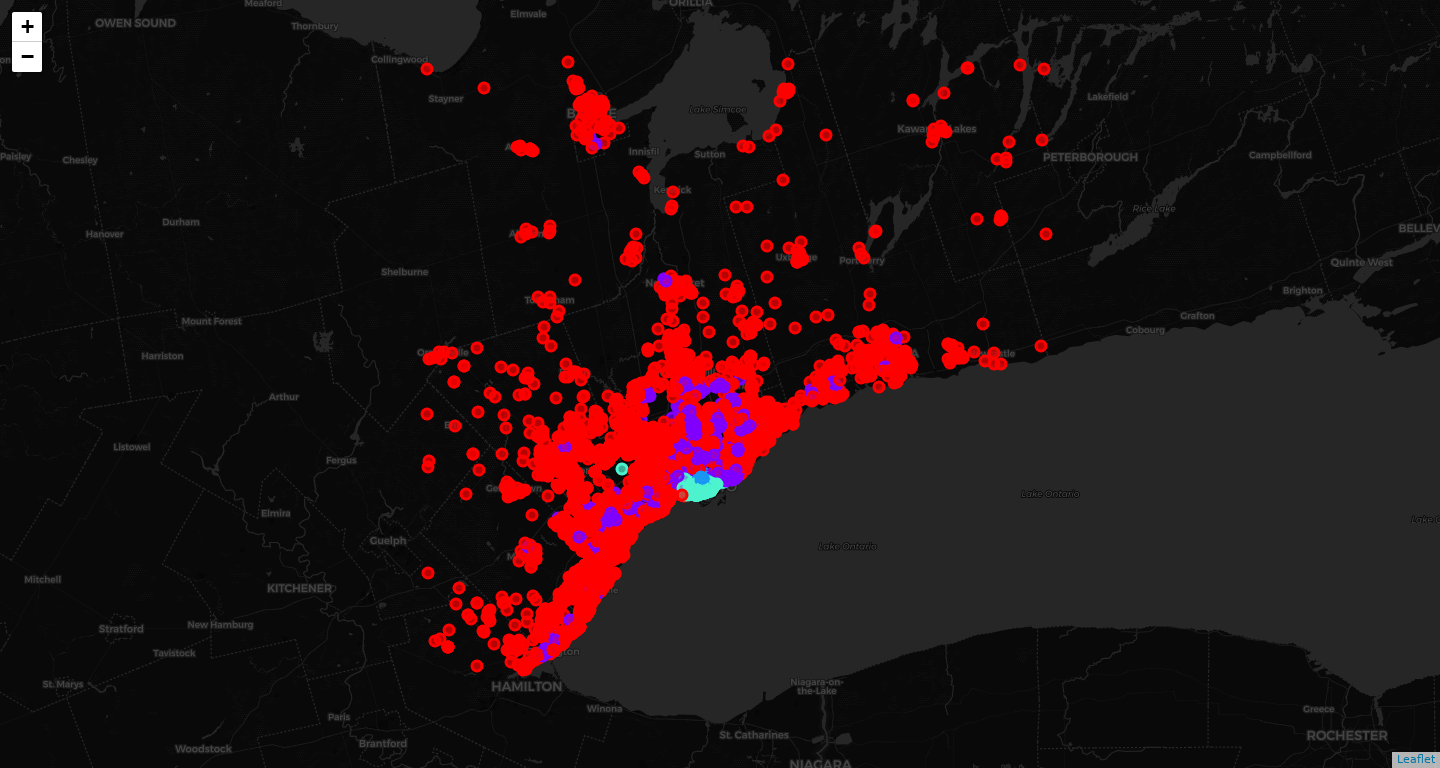
\includegraphics[width=0.85\textwidth]{gta_cluster_map_4.png}
	\caption{Cluster map with k = 4}
	\label{kmeans4}
\end{figure}

\begin{figure}[h]
	\centering
	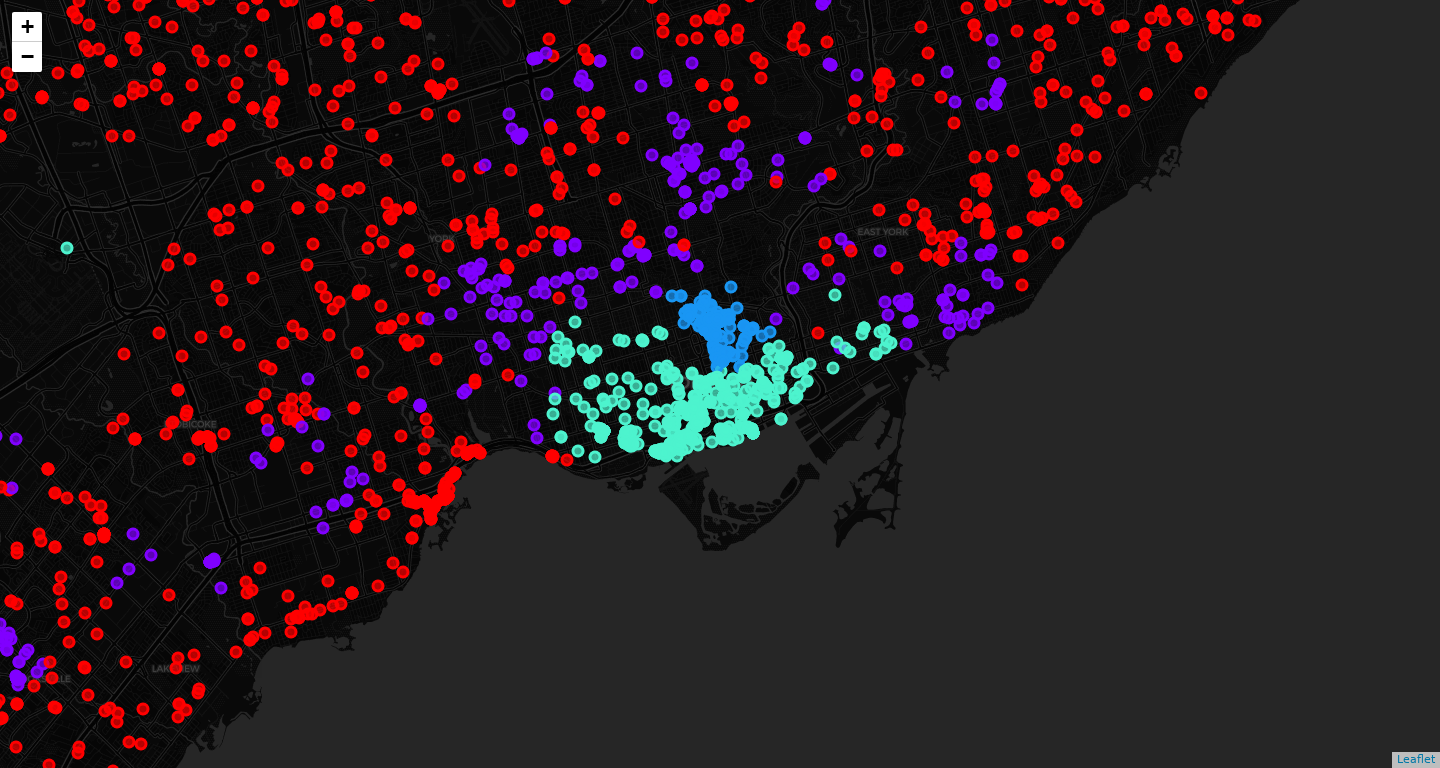
\includegraphics[width=0.85\textwidth]{gta_cluster_map_4_zoom.png}
	\caption{Zoomed in cluster map with k = 4}
	\label{kmeans4zoomed}
\end{figure}

\clearpage
\section{Discussion}

As seen in figure \ref{kmeans4zoomed}, the 4 clusters can clearly be discerned. 

\begin{table}[h!]
	\begin{center}
		\caption{Summary of Clusters}
		\label{tab:table1}
		\vspace{2mm}
		\begin{tabular}{c|c|c} % <-- Alignments: 1st column left, 2nd middle and 3rd right, with vertical lines in between
			\textbf{Cluster labels} & \textbf{Price} & \textbf{Average Venue Distance (m)}\\
			\hline
			0 (red) & \$927,429 & 19621 \\
			1 (purple) & \$675,705 & 58440\\
			2 (blue) & \$860,471 & 64784\\
			3 (turquoise) & \$621,445 & 66562\\
		\end{tabular}
	\end{center}
\end{table}

\begin{itemize}
	\item Cluster 0 can be categorised as upscale suburban housing due to having the highest average price and the scale at which it is spread across the suburbs of the GTA
	\item Cluster 2 can be categorised as upscale downtown housing since it is concentrated primarily around the Yorkville and Rosedale neighbourhoods, two particularly affluent neighbourhoods in Toronto and the GTA
	\item Cluster 1 can be categorised as more affordable suburban housing since it has a lower average price in the suburbs and is not restricted to just downtown
	\item Cluster 3 can be categorised as more affordable downtown housing due to it high concentration in the city of Toronto and having the lower average price.
\end{itemize}

One thing to notice is that the average venue distance seems larger in the case of the downtown locations becuase there are more popular venues around each location, adding to the total distance. Since the k-means algorithm is unsupervised and unlabeled, there is no way to assign a weight to a higher or lower distance, it clusters based on the distance between the points and clusters.


\section{Conclusion}

The k-means unsupervised machine learning clustering algorithm is an effective method in segmenting a city, municipality, or even in this case a metropolitan area. The only difficulties faced in making this analysis was acquiring the right data from a reputable source, which in this case was not possible. Also, obtaining and working with the shapefiles proved to be a difficult task. Aside from these roadblocks, the actual process of creating a machine learning algorithm and analysing the data was a very intuitive process.



\clearpage
\section{Appendix}

\begin{figure}[h]
	\centering
	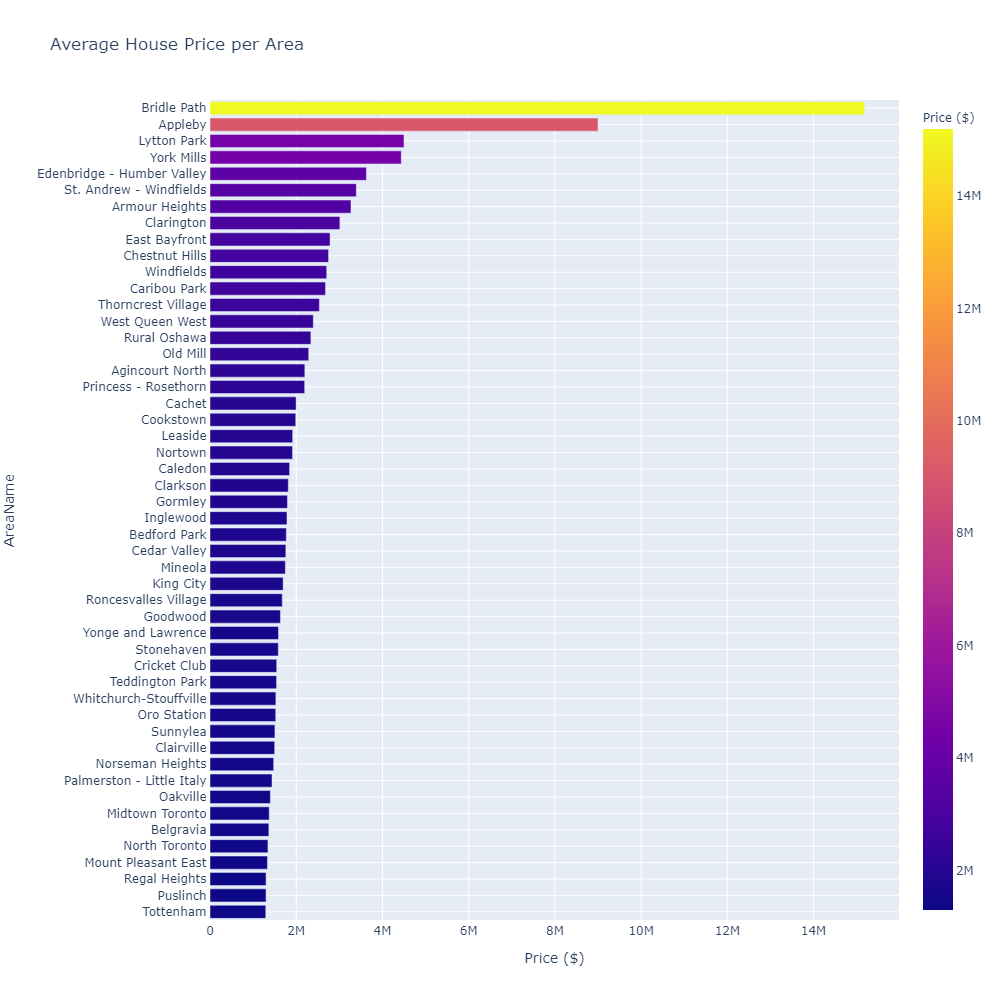
\includegraphics[width=\textwidth]{house-price-plot3.png}
	\caption{Average house price per area}
	\label{price}
\end{figure}


\end{document}

